\documentclass{article}
    % General document formatting
    \usepackage[margin=0.7in]{geometry}
    \usepackage[parfill]{parskip}
    \usepackage[utf8]{inputenc}
    \usepackage{amsmath}
    \usepackage{amssymb}
    \usepackage{tikz}
    \usepackage{fancyhdr}
    \usepackage{listings}
    \usepackage{multicol}
    \usepackage{polynom}

\pagestyle{fancy}
\fancyhf{}
\rhead{Edgar Jacob Rivera Rios - A01184125}

\begin{document}
\begin{titlepage}

    \newcommand{\HRule}{\rule{\linewidth}{0.5mm}} % Defines a new command for the horizontal lines, change thickness here

    \center % Center everything on the page

    %----------------------------------------------------------------------------------------
    %	HEADING SECTIONS
    %----------------------------------------------------------------------------------------

    \textsc{\LARGE Tecnológico de Monterrey}\\[1.5cm] % Name of your university/college
    \textsc{\Large Fundamentos de computación}\\[0.5cm] % Major heading such as course name
    %\textsc{\large Minor Heading}\\[0.5cm] % Minor heading such as course title

    %----------------------------------------------------------------------------------------
    %	TITLE SECTION
    %----------------------------------------------------------------------------------------

    \HRule \\[0.4cm]
    { \huge \bfseries Homework 8}\\[0.4cm] % Title of your document
    \HRule \\[1.5cm]

    %----------------------------------------------------------------------------------------
    %	AUTHOR SECTION
    %----------------------------------------------------------------------------------------

    \begin{minipage}{0.4\textwidth}
    \begin{flushleft} \large
    \emph{Student:}\\
    Jacob \textsc{Rivera} % Your name
    \end{flushleft}
    \end{minipage}
    ~
    \begin{minipage}{0.4\textwidth}
    \begin{flushright} \large
    \emph{Professor:} \\
    Dr. Hugo \textsc{Terashima} % Supervisor's Name
    \end{flushright}
    \end{minipage}\\[2cm]

    % If you don't want a supervisor, uncomment the two lines below and remove the section above
    %\Large \emph{Author:}\\
    %John \textsc{Smith}\\[3cm] % Your name

    %----------------------------------------------------------------------------------------
    %	DATE SECTION
    %----------------------------------------------------------------------------------------

    {\large \today}\\[2cm] % Date, change the \today to a set date if you want to be precise

    %----------------------------------------------------------------------------------------
    %	LOGO SECTION
    %----------------------------------------------------------------------------------------

    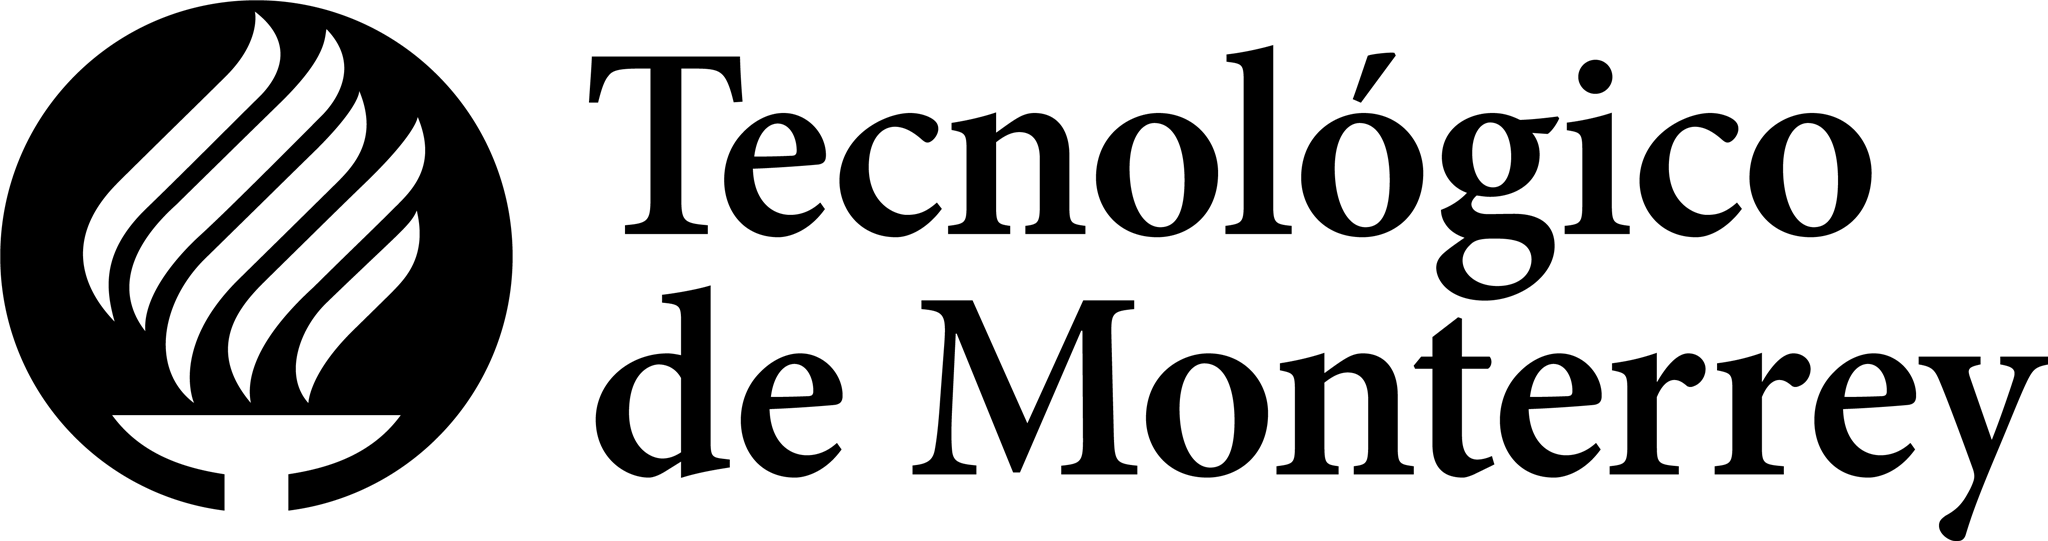
\includegraphics[width=0.4\textwidth,height=\textheight,keepaspectratio]{logo-tec-negro.png} % Include a department/university logo - this will require the graphicx package

    %----------------------------------------------------------------------------------------

    \vfill % Fill the rest of the page with whitespace

\end{titlepage}


\section{Problems}
Solve the following problems:
\begin{enumerate}
    \item Investigate the algorithm for computing the maximum flow on a graph. Provide and example and apply the algorithm, showing each step.


    \item Given a graph $G = (V, E, W)$ and a MST $T$, suppose that we decrease the weight of one of the edges not in $T$. Design an algorithm and its computational complexity to find the MST in the modified graph.

    The simplest way would be to add the edge to the MST, which will provoke for a cycle to be created. After that you just have to search for the biggest edge in that cycle and then remove it. As such, the complexity would be $O(n)$, because in the worst scenario, the cycle would include all the edges of the original MST

    \begin{figure}[ht]
        \centering
        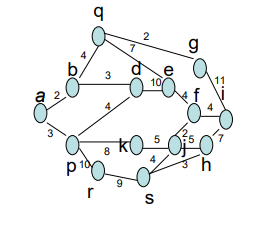
\includegraphics{Hw8/P1.png}
        \caption{Graph}
        \label{graph}
    \end{figure}
    \item Obtain the MST for the graph in Figure 1 using both the Kruskal and Dijkstra/Prim algorithms.

    \textbf{Kruskal}

    Order the edges

    \begin{multicols}{2}
        \begin{center}
        \begin{tabular}{| c | c |}
            \hline
            edge & weight  \\ \hline
            ab & 2  \\
            ap & 3  \\
            bd & 3  \\
            bq & 4  \\
            de & 10 \\
            dp & 4  \\
            ef & 4  \\
            eq & 7  \\
            fi & 4  \\
            fj & 2  \\
            gq & 2  \\
            gi & 11 \\
            hj & 5  \\
            hi & 7  \\
            hs & 3  \\
            jk & 5  \\
            js & 4  \\
            kp & 8  \\
            pr & 10 \\
            rs & 9 \\ \hline
        \end{tabular}

        \columnbreak
        \begin{tabular}{| c | c |}
            \hline
            edge & weight  \\ \hline
            ab & 2  \\
            fj & 2  \\
            gq & 2  \\
            ap & 3  \\
            bd & 3  \\
            hs & 3  \\
            bq & 4  \\
            dp & 4  \\
            ef & 4  \\
            fi & 4  \\
            js & 4  \\
            hj & 5  \\
            jk & 5  \\
            eq & 7  \\
            hi & 7  \\
            kp & 8  \\
            rs & 9 \\
            de & 10 \\
            pr & 10 \\
            gi & 11 \\ \hline
        \end{tabular}
        \end{center}
    \end{multicols}

    Construct the MST by adding the unconnected graphs, from lowest to highest by cost.

    \begin{tabular}{| c | c | c |}
        \hline
        edge & weight & \\ \hline
        ab & 2 & added \\
        fj & 2 & added \\
        gq & 2 & added  \\
        ap & 3 & added \\
        bd & 3 & added \\
        hs & 3 & added \\
        bq & 4 & added \\
        dp & 4 & not added\\
        ef & 4 & added \\
        fi & 4 & added \\
        js & 4 & added \\
        hj & 5 & not added  \\
        jk & 5 & added \\
        eq & 7 & added \\
        hi & 7 & not added \\
        kp & 8 & not added\\
        rs & 9 & added \\
        de & 10 & not added \\
        pr & 10 & not added \\
        gi & 11 & not added \\ \hline
    \end{tabular}
    \begin{figure}[ht]
        \centering
        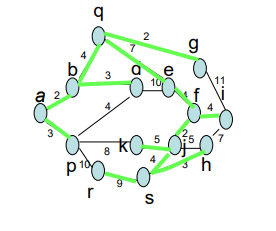
\includegraphics{Hw8/R1.png}
        \caption{MST by Kruskal}
        \label{graph2}
    \end{figure}

    \textbf{Prim–Dijkstra}\\
    Starting conditions:\\
    Start with $a$
    \begin{itemize}
        \item Tree = \{$a$\}
        \item Frontier = $\{b, p\}$
        \item Unvisited = $\{d, e, f, h, i, j, k, q, r, s \}$
        \item MST = $\{\}$
    \end{itemize}
    Final conditions:
    \begin{itemize}
        \item Tree = \{$a, b, d, e, f, h, i, j, k, p, q, r, s$\}
        \item Frontier = $\{\}$
        \item Unvisited = $\{\}$
        \item MST = $\{ab, ap, bd, bq, qg, qe, ef, fj, fi, js, sh, jk, sr\}$
    \end{itemize}

    \begin{figure}[ht]
        \centering
        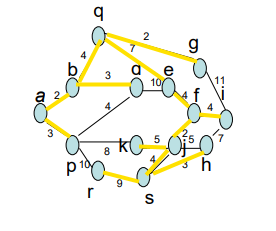
\includegraphics{Hw8/R2.png}
        \caption{MST by Prim–Dijkstra}
        \label{graph3}
    \end{figure}

    \item Design a graph with at least 4 components (biconnected, each with three or more nodes) and run the algorithm seen in class to obtain them. Show the steps.
    \begin{figure}[ht]
        \centering
        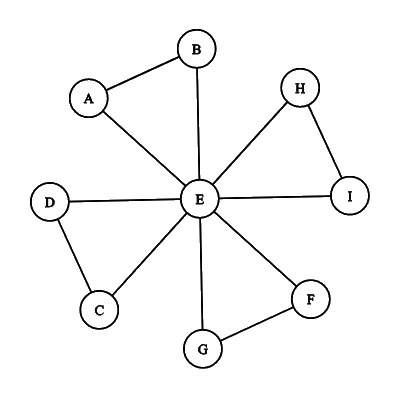
\includegraphics{Hw8/G1.png}
        \caption{4 biconnected components graph}
        \label{graph4}
    \end{figure}

    \begin{itemize}
        \item Star with 1
        \item A $\rightarrow$ (1, 1)
        \item B $\rightarrow$ (2, 2)
        \item E $\rightarrow$ (3, 3)
        \item Find back edge to A
        \item E $\rightarrow$ (3, 1), B $\rightarrow$ (2, 1)
        \item C $\rightarrow$ (4, 4)
        \item D $\rightarrow$ (5, 5)
        \item Find back edge to E
        \item C $\rightarrow$ (4, 3), D $\rightarrow$ (5, 3)
        \item F $\rightarrow$ (6, 6)
        \item G $\rightarrow$ (7, 7)
        \item Find back edge to E
        \item F $\rightarrow$ (6, 3), G $\rightarrow$ (7, 3)
        \item H $\rightarrow$ (8, 8)
        \item I $\rightarrow$ (9, 9)
        \item Find back edge to E
        \item H $\rightarrow$ (8, 3), I $\rightarrow$ (9, 3)
    \end{itemize}

    \begin{figure}[ht]
        \centering
        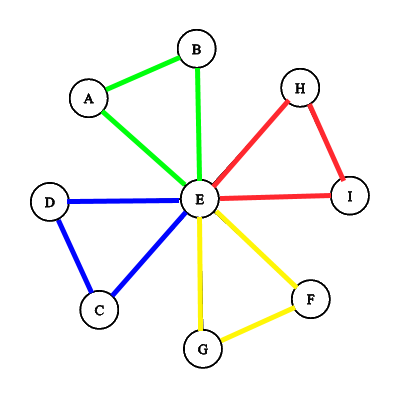
\includegraphics{Hw8/G2.png}
        \caption{5 biconnected components graph colored}
        \label{graph5}
    \end{figure}

    \pagebreak
    \item Design a directed graph and establish an origin and a destination and apply the algorithm Dijkstra/Prim to obtain the shortest path between both nodes. Show the steps.

    \begin{figure}[ht]
        \centering
        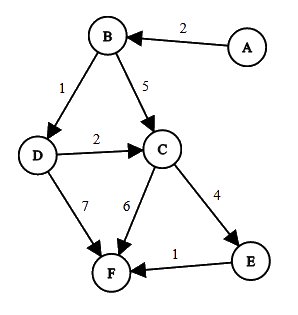
\includegraphics{Hw8/G3.png}
        \caption{Graph for shortest path}
        \label{graph6}
    \end{figure}

    Get a shortest path from $A$ to $F$

    \begin{itemize}
        \item Open = $\{(A,0)\}$, Frontier=$\{(B,2)\}$, Closed=$\{(C,\infty),(D,\infty), (E,\infty), (F,\infty)\}$
        \item Open = $\{(A,0), (B,2)\}$, Frontier=$\{(C,7),(D,3)\}$, Closed=$\{(E,\infty),(F,\infty)\}$
        \item Open = $\{(A,0), (B,2), (D,3)\}$, Frontier=$\{(C,5),(F,10)\}$, Closed=$\{(E,\infty)\}$
        \item Open = $\{(A,0), (B,2), (D,3), (C,5)\}$, Frontier=$\{(E,9),(F,10)\}$, Closed=$\{\}$
        \item Open = $\{(A,0), (B,2), (D,3), (C,5), (E,9)\}$, Frontier=$\{(F,10)\}$, Closed=$\{\}$
        \item Open = $\{(A,0), (B,2), (D,3), (C,5), (E,9), (F,10)\}$, Frontier=$\{\}$, Closed=$\{\}$
    \end{itemize}
    Shortest path is $A \rightarrow B \rightarrow D \rightarrow F$, alternate same length route is $A \rightarrow B \rightarrow D \rightarrow C \rightarrow E \rightarrow F$
\end{enumerate}
\end{document}